\documentclass{beamer}
\usetheme[rule,leftframetitle]{Amurmaple}

% Packages
\usepackage[utf8]{inputenc}
\usepackage[T1]{fontenc}
\usepackage{lmodern}
\usepackage{listings}
\usepackage{xcolor}
\usepackage{tikz}
\usetikzlibrary{shapes,arrows,positioning}

% Code listing settings
\lstset{
  basicstyle=\ttfamily\small,
  keywordstyle=\color{blue}\bfseries,
  commentstyle=\color{gray}\itshape,
  stringstyle=\color{red},
  showstringspaces=false,
  breaklines=true,
  frame=single,
  numbers=left,
  numberstyle=\tiny\color{gray},
  backgroundcolor=\color{gray!10}
}

% Metadata
\title{Technical Presentation}
\subtitle{System Architecture and Implementation}
\author{Technical Team}
\institute{Engineering Department}
\date{\today}

\mail{tech@company.com}

\begin{document}

% Title
\frame{\titlepage}

% Agenda
\begin{frame}{Agenda}
  \tableofcontents
\end{frame}

% Overview
\section{System Overview}

\sepframe

\begin{frame}{Architecture Overview}
  \begin{center}
    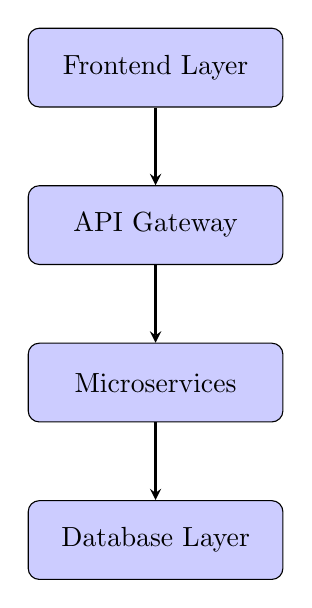
\begin{tikzpicture}[
      node distance=2cm,
      block/.style={rectangle, draw, fill=blue!20, text width=3cm, text centered, rounded corners, minimum height=1cm},
      arrow/.style={thick,->,>=stealth}
    ]
      \node [block] (frontend) {Frontend Layer};
      \node [block, below of=frontend] (api) {API Gateway};
      \node [block, below of=api] (services) {Microservices};
      \node [block, below of=services] (database) {Database Layer};

      \draw [arrow] (frontend) -- (api);
      \draw [arrow] (api) -- (services);
      \draw [arrow] (services) -- (database);
    \end{tikzpicture}
  \end{center}
\end{frame}

\begin{frame}{Technology Stack}
  \begin{columns}[T]
    \begin{column}{0.48\textwidth}
      \framesection{Frontend}
      \begin{itemize}
        \item React 18
        \item TypeScript
        \item TailwindCSS
        \item Redux Toolkit
      \end{itemize}

      \framesection{Backend}
      \begin{itemize}
        \item Node.js 20
        \item Express.js
        \item PostgreSQL
        \item Redis
      \end{itemize}
    \end{column}
    \begin{column}{0.48\textwidth}
      \framesection{Infrastructure}
      \begin{itemize}
        \item Docker
        \item Kubernetes
        \item AWS ECS
        \item GitHub Actions
      \end{itemize}

      \framesection{Monitoring}
      \begin{itemize}
        \item Prometheus
        \item Grafana
        \item Sentry
        \item CloudWatch
      \end{itemize}
    \end{column}
  \end{columns}
\end{frame}

% Implementation
\section{Implementation Details}

\sepframe

\begin{frame}[fragile]{API Endpoint Example}
  \framesection{User Authentication}

  \begin{lstlisting}[language=JavaScript]
// POST /api/auth/login
app.post('/api/auth/login', async (req, res) => {
  const { email, password } = req.body;

  // Validate input
  const user = await User.findByEmail(email);
  if (!user) {
    return res.status(401).json({
      error: 'Invalid credentials'
    });
  }

  // Verify password
  const isValid = await bcrypt.compare(
    password,
    user.passwordHash
  );

  if (isValid) {
    const token = jwt.sign({ userId: user.id });
    return res.json({ token });
  }

  return res.status(401).json({
    error: 'Invalid credentials'
  });
});
  \end{lstlisting}
\end{frame}

\begin{frame}[fragile]{Database Schema}
  \framesection{Users Table}

  \begin{lstlisting}[language=SQL]
CREATE TABLE users (
  id SERIAL PRIMARY KEY,
  email VARCHAR(255) UNIQUE NOT NULL,
  password_hash VARCHAR(255) NOT NULL,
  first_name VARCHAR(100),
  last_name VARCHAR(100),
  created_at TIMESTAMP DEFAULT CURRENT_TIMESTAMP,
  updated_at TIMESTAMP DEFAULT CURRENT_TIMESTAMP,
  last_login TIMESTAMP,
  is_active BOOLEAN DEFAULT true,

  CONSTRAINT email_format
    CHECK (email ~* '^[A-Za-z0-9._%+-]+@[A-Za-z0-9.-]+\.[A-Z|a-z]{2,}$')
);

CREATE INDEX idx_users_email ON users(email);
CREATE INDEX idx_users_active ON users(is_active);
  \end{lstlisting}
\end{frame}

\begin{frame}[fragile]{Docker Configuration}
  \framesection{Dockerfile}

  \begin{lstlisting}[language=Docker]
FROM node:20-alpine AS builder

WORKDIR /app
COPY package*.json ./
RUN npm ci --only=production

COPY . .
RUN npm run build

# Production stage
FROM node:20-alpine
WORKDIR /app

COPY --from=builder /app/dist ./dist
COPY --from=builder /app/node_modules ./node_modules
COPY package*.json ./

EXPOSE 3000
CMD ["node", "dist/server.js"]
  \end{lstlisting}
\end{frame}

% Deployment
\section{Deployment Process}

\sepframe

\begin{frame}{CI/CD Pipeline}
  \framesection{Automated Workflow}

  \begin{enumerate}
    \item \textbf{Code Push} - Developer pushes to GitHub
    \item \textbf{Build} - GitHub Actions builds Docker image
    \item \textbf{Test} - Run unit and integration tests
    \item \textbf{Security Scan} - Vulnerability scanning
    \item \textbf{Deploy to Staging} - Automatic deployment
    \item \textbf{E2E Tests} - Run end-to-end tests
    \item \textbf{Manual Approval} - Team review
    \item \textbf{Deploy to Production} - Blue-green deployment
  \end{enumerate}
\end{frame}

\begin{frame}{Deployment Strategy}
  \begin{block}{Blue-Green Deployment}
    \begin{itemize}
      \item Maintain two identical production environments
      \item Deploy new version to inactive environment (green)
      \item Run smoke tests on green environment
      \item Switch traffic from blue to green
      \item Keep blue as rollback option
    \end{itemize}
  \end{block}

  \begin{alertblock}{Rollback Procedure}
    If issues detected:
    \begin{enumerate}
      \item Stop accepting new requests
      \item Switch traffic back to blue
      \item Investigate and fix issues
      \item Re-deploy when ready
    \end{enumerate}
  \end{alertblock}
\end{frame}

% Performance
\section{Performance Metrics}

\sepframe

\begin{frame}{System Performance}
  \framesection{Key Metrics}

  \begin{table}
    \centering
    \begin{tabular}{lcc}
      \toprule
      Metric & Target & Current \\
      \midrule
      Response Time (p95) & < 200ms & 156ms \\
      Throughput & 1000 req/s & 1250 req/s \\
      Error Rate & < 0.1\% & 0.05\% \\
      Uptime & 99.9\% & 99.95\% \\
      \bottomrule
    \end{tabular}
  \end{table}

  \begin{exampleblock}{Optimization Results}
    \begin{itemize}
      \item 40\% reduction in database queries
      \item Redis caching reduced latency by 60\%
      \item CDN integration improved static asset delivery
    \end{itemize}
  \end{exampleblock}
\end{frame}

% Security
\section{Security Considerations}

\sepframe

\begin{frame}{Security Measures}
  \framesection{Authentication \& Authorization}

  \begin{itemize}
    \item JWT-based authentication
    \item Role-based access control (RBAC)
    \item OAuth 2.0 integration
    \item Multi-factor authentication (MFA)
  \end{itemize}

  \framesection{Data Protection}

  \begin{itemize}
    \item TLS 1.3 encryption in transit
    \item AES-256 encryption at rest
    \item Secure credential storage (AWS Secrets Manager)
    \item Regular security audits
  \end{itemize}
\end{frame}

% Future Work
\section{Future Enhancements}

\sepframe

\begin{frame}{Roadmap}
  \begin{information}[Q1 2025]
    \begin{itemize}
      \item GraphQL API implementation
      \item Real-time WebSocket support
      \item Enhanced monitoring dashboard
    \end{itemize}
  \end{information}

  \begin{information}[Q2 2025]
    \begin{itemize}
      \item Kubernetes migration
      \item Service mesh implementation (Istio)
      \item Machine learning model integration
    \end{itemize}
  \end{information}
\end{frame}

% Conclusion
\section{Conclusion}

\sepframe

\begin{frame}{Summary}
  \begin{enumerate}
    \item Robust microservices architecture
    \item Automated CI/CD pipeline
    \item Strong security measures
    \item Excellent performance metrics
    \item Clear roadmap for future enhancements
  \end{enumerate}

  \bigskip

  \begin{block}{Resources}
    \begin{itemize}
      \item Documentation: \url{https://docs.company.com}
      \item Source Code: \url{https://github.com/company/project}
      \item Contact: tech@company.com
    \end{itemize}
  \end{block}
\end{frame}

% Questions
\thanksframe{Questions?}

\end{document}
